\documentclass[conference]{IEEEtran}

\usepackage{cite}
\usepackage{amsmath,amssymb,amsfonts}
\DeclareMathOperator*{\argmax}{argmax}
\DeclareMathOperator*{\argmin}{argmin}
\DeclareMathOperator{\Tr}{Tr}
\DeclareMathOperator{\veco}{vec}
\DeclareMathOperator{\Tdiag}{T_{diag}}
\usepackage{algorithmic}
\usepackage{graphicx}
\usepackage{textcomp}
\usepackage{xcolor}
\usepackage{tikz}
\usepackage{comment}
\def\BibTeX{{\rm B\kern-.05em{\sc i\kern-.025em b}\kern-.08em
    T\kern-.1667em\lower.7ex\hbox{E}\kern-.125emX}}
\begin{document}

\title{My Ideas}

\author{\IEEEauthorblockN{Jonathan Lane}}

\maketitle

\begin{abstract}
Just me talkin % don't worry bout nothin
\end{abstract}

\section{Introduction}
This document aims to inform the reader about my current ideas on the relationship between network theory and the connections between rigid bodies and their states. It has been observed that the mass matrix $M$ in the Euler-Lagrange equation resembles that of the graph Laplacian of an undirected graph. My research focuses on the network interpretation of a single robotic system which may lead to further research in modeling the connections of rigid bodies algebraically.

\section{Setup}

\begin{figure}[htbp]
    \centering
    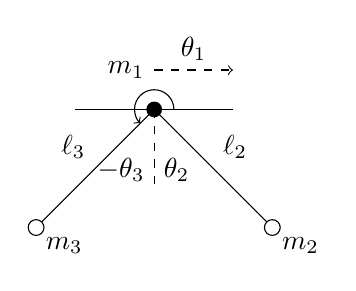
\begin{tikzpicture}
        \draw (-1, 0) -- (1, 0);
        \fill[black] (0, 0) circle (1mm);
        \draw[->] (0.25, 0) arc (0:225:2.5mm);
        \draw[->, dashed] (0, 0.5) node[anchor=east] {$m_1$} -- node[anchor=south] {$\theta_1$} (1, 0.5);
        \draw[dashed] (0, 0) -- node[anchor=north west] {$\theta_2$} node[anchor=north east] {$-\theta_3$} (0, -1);
        
        \draw (0, 0) -- node[anchor=south west] {$\ell_2$} (1.5, -1.5);
        \filldraw[fill=white, draw=black] (1.5, -1.5) circle (1mm) node[anchor=north west] {$m_2$};
        
        \draw (0, 0) -- node[anchor=south east] {$\ell_3$} (-1.5, -1.5);
        \filldraw[fill=white, draw=black] (-1.5, -1.5) circle (1mm) node[anchor=north west] {$m_3$};
    \end{tikzpicture}
    \caption{Mechanical diagram for two single pendulums on a cart}
    \label{fig:ssp_diagram}
\end{figure}

Let the following equation be a simplified for of the Euler-Lagrange equation which represents the dynamics of a general robotic system:
$$
M(\theta)\ddot{\theta}=f(\dot{\theta},\theta)
$$
where $M(\theta)$ is the mass matrix and $f(\dot{\theta},\theta)$ is the sum of the coriolis and gravitational terms. It can be shown that the mass matrix is always symmetric and positive definite for any system described in this way, thus $M(\theta)$ is invertible:
\begin{equation}
    \label{dynamics_eq}
    \ddot{\theta}=M(\theta)^{-1}f(\dot{\theta},\theta)
\end{equation}

Now consider the consensus equation expressed with the graph Laplacian:
$$
\dot{x}=-L(\mathcal{D})x
$$
This is the form that I wish to compare to \eqref{dynamics_eq} to understand a graph theoretical meaning of the mass and inertial relationships between rigid bodies. The idea is that the network connections represented in the graph Laplacian are encoded in the mass matrix somehow. Let's examine $M(\theta)$ and $M(\theta)^{-1}$ for the system of two pendulums on a cart as shown in Figure \ref{fig:ssp_diagram}:
$$
M(\theta)=\left[\begin{matrix}m_{1} + m_{2} + m_{3} & l_{2} m_{2} \cos{\theta_2} & l_{3} m_{3} \cos{\theta_3}\\l_{2} m_{2} \cos{\theta_2} & l_{2}^{2} m_{2} & 0\\l_{3} m_{3} \cos{\theta_3} & 0 & l_{3}^{2} m_{3}\end{matrix}\right]
$$
$$
M(\theta)^{-1}=\frac{1}{d}\begin{bmatrix}
    1 & - \frac{\cos{\theta_2}}{l_{2}} & - \frac{\cos{\theta_3}}{l_{3}}\\
    -\frac{\cos{\theta_2}}{l_{2}} & \frac{m_{1} + m_{2} + m_{3} \sin^{2}{\theta_2}}{l_{2}^{2} m_{2}} & \frac{\cos{\theta_2} \cos{\theta_3}}{l_{2} l_{3}}\\
    - \frac{\cos{\theta_3}}{l_{3}} & \frac{\cos{\theta_2} \cos{\theta_3}}{l_{2} l_{3}} & \frac{m_{1} + m_{2} \sin^{2}{\theta_2} + m_{3}}{l_{3}^{2} m_{3}}
\end{bmatrix}
$$
$$
d=m_{1} + m_{2} \sin^{2}{\theta_2} + m_{3} \sin^{2}{\theta_3}
$$
where $d$ is a common denominator within $M(\theta)^{-1}$. Although, matrices are symmetric, this doesn't show that there is a mathematical link between rigid bodies. In the following sections, we will examine the decomposition of $M(\theta)^{-1}$.

Finally, let us formulate a graph which we expect to represent the two pendulum system. Let nodes $(v_1, v_2, v_3)$ correspond to bodies 1, 2, and 3 in Figure 1. We expect an edge to exist between the pairs $(v_1, v_2)$ and $(v_1, v_3)$ because they are physically connected, and no edge between $(v_2, v_3)$ because they are not. Also, the graph will be defined as undirected, because we do not yet know the direction of information flow within the graph. Furthermore, the Laplacian of an undirected graph is symmetric, which it will need to be to compare with $M(\theta)$ or $M(\theta)^{-1}$.

\begin{figure}[htbp]
    \centering
    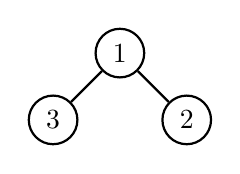
\begin{tikzpicture}[node distance={12mm}, thick, main/.style = {draw, circle}]
        \node[main] (1) {$1$};
        \node[main] (2) [below right of=1] {$2$};
        \node[main] (3) [below left of=1] {$3$};
        \draw (1) -- (2);
        \draw (1) -- (3);
    \end{tikzpicture}
    \caption{Estimated graph for two pendulum system}
    \label{ssp_graph}
\end{figure}

$$
L(\mathcal{G}) = \begin{bmatrix}
    2 & -1 & -1\\
    -1 & 1 & 0\\
    -1 & 0 & 1
\end{bmatrix}
$$
$L(\mathcal{G})$ is the graph Laplacian for the undirected graph in Figure \ref{fig:ssp_diagram}. It is important to note that a zero entry in the $(i,j)$ position indicates the nonexistence of an edge between nodes $i$ and $j$.

\section{Definitions}

\noindent\textbf{Definition 1.} For a digraph $\mathcal{D}$, the incidence matrix $D(\mathcal{D})\in\mathbb{R}^{n\times m}$ is a matrix defined as follows:
$$
D(\mathcal{D})=\left[d_{ij}\right],\text{where }d_{ij}=
\begin{cases}
    -1 & \text{if }v_i\text{ is the tail of }e_j\\
    1 & \text{if }v_i\text{ is the head of }e_j\\
    0 & otherwise
\end{cases}
$$
where $v_i$ is the ith vertex of $\mathcal{G}$ and $e_j$ is the jth edge. The incidence matrix captures the features of the edges of a graph and the vertices they connect to.
One important feature of the incidence matrix is that each column describes one edge, so each column has one $-1$ and one $1$, and $\mathbf{1}\in\mathcal{N}(D(\mathcal{D})^T)$.

\noindent\textbf{Definition 2.} The graph Laplacian of $\mathcal{G}$, the undirected version of $\mathcal{D}$, can be defined as:
$$
L(\mathcal{G})=D(\mathcal{D})D(\mathcal{D})^T
$$
which describes the connections between nodes in the graph.

\noindent\textbf{Definition 3.} The edge Laplacian of $\mathcal{G}$ is defined as:
$$
L_e(\mathcal{G})=D(\mathcal{D})^TD(\mathcal{D})
$$
which describes the connections between edges in the graph.

\noindent\textbf{Definition 4.} The Cholesky decomposition of a symmetric positive-definite matrix is written as:
$$
A=LL^T
$$
where L is a real lower triangular matrix with positive diagonal entries. This decomposition can also be done with upper triangular matrices such that $A=UU^T$.

\section{Decomposition of the Inverse Mass Matrix}

\subsection{Two Pendulums on a Cart}
Let the Cholesky decomposition of $M(\theta)^{-1}$ be defined as:
$$
M(\theta)^{-1}=L(\theta)L(\theta)^T
$$
For the two pendulum system described above, $L(\theta)$ is:
$$
L(\theta)=\left[\begin{matrix}
    \frac{1}{\sqrt{d}} & 0 & 0\\
    -\frac{\cos{\theta_2}}{l_{2} \sqrt{d}} & \frac{1}{l_2 \sqrt{m_2}} & 0\\
    -\frac{\cos{\theta_3}}{l_{3} \sqrt{d}} & 0 & \frac{1}{l_3 \sqrt{m_3}}
\end{matrix}\right]
$$
Finally, something interesting happens if we evaluate $L(\theta)^TL(\theta)$:
$$
L(\theta)^TL(\theta)=\left[\begin{matrix}
    \frac{l_2^2 l_3^2 + l_2^2 \cos^2\theta_3 + l_3^2 \cos^2\theta_2}{l_2^2 l_3^2 d} & -\frac{\cos\theta_2}{l_2^2 \sqrt{m_2 d}} & - \frac{\cos\theta_3}{l_3^2 \sqrt{m_3 d}}\\
    -\frac{\cos\theta_2}{l_2^2 \sqrt{m_2 d}} & \frac{1}{l_2^2 m_2} & 0\\
    -\frac{\cos\theta_3}{l_3^2 \sqrt{m_3 d}} & 0 & \frac{1}{l_3^2 m_3}
\end{matrix}\right]
$$
We see that the structure is similar to the expected graph Laplacian $L(\mathcal{G})$! The idea here is that $L(\theta)$ is related to some incidence matrix $D(\mathcal{D})^T$, and $M(\theta)^{-1}$ is related to some edge Laplacian $L_e(\mathcal{G})$ with states $\theta$. Therefore, the graph theoretical links between rigid bodies in a robotic system do not exist in terms of $\theta$, but in terms of the edges of the underlying graph. However, none of this matters if it is not generalizable to all robotic systems, or at least those that satisfy some given conditions. Let's look at a couple more examples.

\subsection{Double and Single Pendulums on a Cart}
\begin{figure}[htbp]
    \centering
    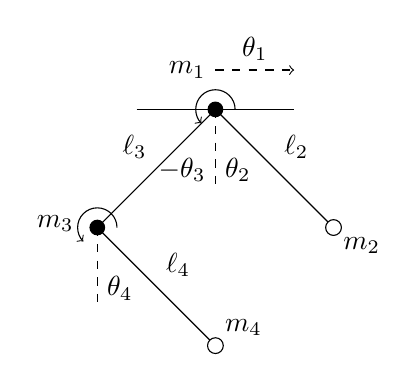
\begin{tikzpicture}
        \draw (-1, 0) -- (1, 0);
        \fill[black] (0, 0) circle (1mm);
        \draw[->] (0.25, 0) arc (0:225:2.5mm);
        \draw[->, dashed] (0, 0.5) node[anchor=east] {$m_1$} -- node[anchor=south] {$\theta_1$} (1, 0.5);
        \draw[dashed] (0, 0) -- node[anchor=north west] {$\theta_2$} node[anchor=north east] {$-\theta_3$} (0, -1);
        
        \draw (0, 0) -- node[anchor=south west] {$\ell_2$} (1.5, -1.5);
        \filldraw[fill=white, draw=black] (1.5, -1.5) circle (1mm) node[anchor=north west] {$m_2$};
        
        \draw (0, 0) -- node[anchor=south east] {$\ell_3$} (-1.5, -1.5);
        \fill[black] (-1.5, -1.5) circle (1mm);
        \draw[->] (-1.25, -1.5) arc (0:225:2.5mm) node[anchor=south east] {$m_3$};
        \draw[dashed] (-1.5, -1.5) -- node[anchor=north west] {$\theta_4$} (-1.5, -2.5);
        
        \draw (-1.5, -1.5) -- node[anchor=south west] {$\ell_4$} (0, -3);
        \filldraw[fill=white, draw=black] (0, -3) circle (1mm) node[anchor=south west] {$m_4$};
        
    \end{tikzpicture}
    \caption{Mechanical diagram for the double/single pendulum on a cart}
    \label{fig:dsp_diagram}
\end{figure}

\begin{figure}[htbp]
    \centering
    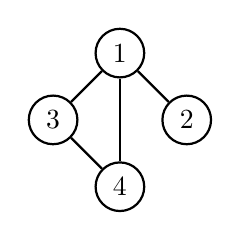
\begin{tikzpicture}[node distance={12mm}, thick, main/.style = {draw, circle}]
        \node[main] (1) {$1$};
        \node[main] (2) [below right of=1] {$2$};
        \node[main] (3) [below left of=1] {$3$};
        \node[main] (4) [below right of=3] {$4$};
        \draw (1) -- (2);
        \draw (1) -- (3);
        \draw (3) -- (4);
        \draw (1) -- (4);
    \end{tikzpicture}
    \caption{Estimated graph for double/single pendulum system}
    \label{dsp_graph}
\end{figure}

Figures \ref{fig:dsp_diagram} and \ref{dsp_graph} show the diagram and estimated graph for the system of two carts sliding on a platform connected to a
pendulum. When we complete similar analysis as before we get $M(\theta)$ to be similar in structure to $L(\mathcal{G})$ like before (not shown, too big to fit).
$$
L(\mathcal{G})=\begin{bmatrix}
    3 & -1 & -1 & -1\\
    -1 & 1 & 0 & 0\\
    -1 & 0 & 2 & -1\\
    -1 & 0 & -1 & 2\\
\end{bmatrix}
$$
$L(\mathcal{G})$ is the graph Laplacian for the undirected graph in Figure \ref{dsp_graph}. $L(\theta)^TL(\theta)$ is a very complicated matrix, so only the structure is shown:
$$
L(\theta)^TL(\theta)=\begin{bmatrix}
    * & * & * & *\\
    * & * & 0 & 0\\
    * & 0 & * & *\\
    * & 0 & * & *
\end{bmatrix}
$$
where $*$ represents a generally nonzero value. Again, the zero entries, which denote the nonexistence of an edge in the graph Laplacian, are consistent between $M(\theta)$, $L(\mathcal{G})$, and $L(\theta)^TL(\theta)$.

\subsection{Two Carts on a Pendulum}
\begin{figure}[htbp]
    \centering
    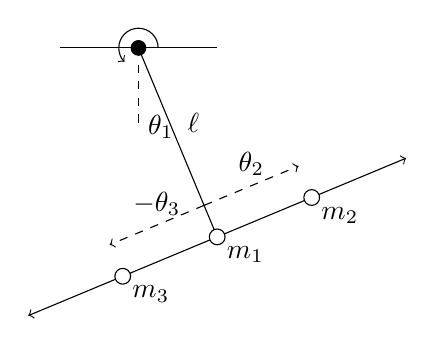
\begin{tikzpicture}
        \draw (-1, 0) -- (1, 0);
        \fill[black] (0, 0) circle (1mm);
        \draw[->] (0.25, 0) arc (0:225:2.5mm);
        \draw (0, 0) -- node[anchor=south west] {$\ell$} (1, -2.4);
        \draw[dashed] (0, 0) -- (0, -1) node[anchor=west] {$\theta_1$};
        
        \draw[->] (1, -2.4) -- (1+2.4, -2.4+1);
        \draw[->] (1, -2.4) -- (1-2.4, -2.4-1);
        \filldraw[fill=white, draw=black] (1, -2.4) circle (1mm) node[anchor=north west] {$m_1$};
        \filldraw[fill=white, draw=black] (1+1.2, -2.4+0.5) circle (1mm) node[anchor=north west] {$m_2$};
        \filldraw[fill=white, draw=black] (1-1.2, -2.4-0.5) circle (1mm) node[anchor=north west] {$m_3$};
        \draw[->, dashed] (5/6, -2) -- node[anchor=south] {$\theta_2$} (5/6+1.2, -2+0.5);
        \draw[->, dashed] (5/6, -2) -- node[anchor=south] {$-\theta_3$} (5/6-1.2, -2-0.5);
    \end{tikzpicture}
    \caption{Mechanical diagram for two carts on a pendulum}
    \label{fig:ccp1_diagram}
\end{figure}

\begin{figure}[htbp]
    \centering
    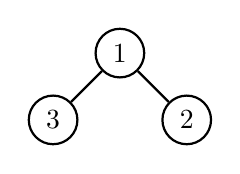
\begin{tikzpicture}[node distance={12mm}, thick, main/.style = {draw, circle}]
        \node[main] (1) {$1$};
        \node[main] (2) [below right of=1] {$2$};
        \node[main] (3) [below left of=1] {$3$};
        \draw (1) -- (2);
        \draw (1) -- (3);
    \end{tikzpicture}
    \caption{Estimated graph for two carts on a pendulum system}
    \label{ccp1_graph}
\end{figure}

Figures \ref{fig:ccp1_diagram} and \ref{ccp1_graph} show the diagram and estimated graph for the system of two carts sliding on a platform connected to a pendulum. When we complete similar analysis as before we get:
$$
M(\theta)=\begin{bmatrix}l^{2} \left(m_{1} + m_{2} + m_{3}\right) + m_{2} \theta_{2}^{2} + m_{3} \theta_{3}^{2} & l m_{2} & l m_{3}\\l m_{2} & m_{2} & 0\\l m_{3} & 0 & m_{3}\end{bmatrix}
$$
$$
L(\theta)^TL(\theta)=\begin{bmatrix}
    * & * & *\\
    * & * & 0\\
    * & 0 & *
\end{bmatrix}
$$

Now, what if we redefine the positions of the $\theta s$, masses, and nodes of the system? Let's see what happens if we switch nodes 1 and 3.
\begin{figure}[htbp]
    \centering
    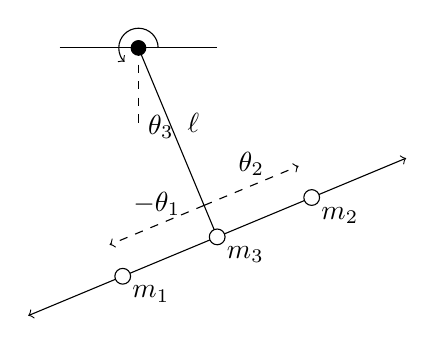
\begin{tikzpicture}
        \draw (-1, 0) -- (1, 0);
        \fill[black] (0, 0) circle (1mm);
        \draw[->] (0.25, 0) arc (0:225:2.5mm);
        \draw (0, 0) -- node[anchor=south west] {$\ell$} (1, -2.4);
        \draw[dashed] (0, 0) -- (0, -1) node[anchor=west] {$\theta_3$};
        
        \draw[->] (1, -2.4) -- (1+2.4, -2.4+1);
        \draw[->] (1, -2.4) -- (1-2.4, -2.4-1);
        \filldraw[fill=white, draw=black] (1, -2.4) circle (1mm) node[anchor=north west] {$m_3$};
        \filldraw[fill=white, draw=black] (1+1.2, -2.4+0.5) circle (1mm) node[anchor=north west] {$m_2$};
        \filldraw[fill=white, draw=black] (1-1.2, -2.4-0.5) circle (1mm) node[anchor=north west] {$m_1$};
        \draw[->, dashed] (5/6, -2) -- node[anchor=south] {$\theta_2$} (5/6+1.2, -2+0.5);
        \draw[->, dashed] (5/6, -2) -- node[anchor=south] {$-\theta_1$} (5/6-1.2, -2-0.5);
    \end{tikzpicture}
    \caption{Mechanical diagram for two carts on a pendulum}
    \label{fig:ccp3_diagram}
\end{figure}

\begin{figure}[htbp]
    \centering
    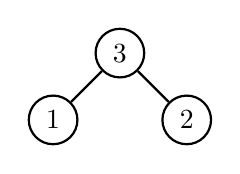
\begin{tikzpicture}[node distance={12mm}, thick, main/.style = {draw, circle}]
        \node[main] (1) {$3$};
        \node[main] (2) [below right of=1] {$2$};
        \node[main] (3) [below left of=1] {$1$};
        \draw (1) -- (2);
        \draw (1) -- (3);
    \end{tikzpicture}
    \caption{Estimated graph for two carts on a pendulum system}
    \label{ccp3_graph}
\end{figure}

We can see the modified diagram and graph in Figures \ref{fig:ccp3_diagram} and \ref{ccp3_graph}. Now, let's recalculate the mass matrix and $L(\theta)^TL(\theta)$ for this redefined system:
$$
M(\theta)=\begin{bmatrix}m_{1} & 0 & l m_{1}\\0 & m_{2} & l m_{2}\\l m_{1} & l m_{2} & l^{2} \left(m_{1} + m_{2} + m_{3}\right) + m_{1} \theta_{1}^{2}{\left(t \right)} + m_{2} \theta_{2}^{2}{\left(t \right)}\end{bmatrix}
$$
$$
L(\theta)^TL(\theta)=\begin{bmatrix}
    * & * & *\\
    * & * & *\\
    * & * & *
\end{bmatrix}
$$
The mass matrix is what we expect, indicating no edge between 1 and 2, but the edge Laplacian does not have zero entries anywhere! This is due to the way the Cholesky decomposition is defined, there is no way (I think) to get zeros \textit{only} in the $(1,2)$ and $(2,1)$ positions from the product of a lower and an upper triangular matrix (in that order). However, we can actually define the Cholesky decomposition as the product of an upper triangular matrix and its transpose by performing the algorithm starting from the bottom right of the matrix rather than the upper left. Let's define the upper triangular version as:
$$
M(\theta)^{-1}=U(\theta)U(\theta)^T
$$
Now, by doing this version of the decomposition, and switching the order, we get:
$$
U(\theta)^TU(\theta)=\begin{bmatrix}
    * & * & *\\
    * & * & 0\\
    * & 0 & *
\end{bmatrix}
$$
which is what we expect! The final permutation of defining this system is to make node 2 the pendulum that the carts are connected to, in other words, make node 2 the root of the graph. The algorithm yields matrices with all nonzero elements for both $L(\theta)^TL(\theta)$ and $U(\theta)^TU(\theta)$.

\section{Conclusions}
\begin{itemize}
    \item If all nonzero values exist along the diagonal, first row, and first column of $M(\theta)$, the matrix $L(\theta)^TL(\theta)$ derived from the Cholesky decomposition of $M(\theta)^{-1}$ resembles the structure of the mass matrix $M(\theta)$.
    \item To make the first row and column of $L(\theta)^TL(\theta)$ contain no zeros, $\theta_1$ must define the position of the body that is "linked" to all other bodies, or in other words, node 1 must have edges that connect to all other nodes.
    \item There may exist another decomposition that can generalize the similarity between $M(\theta)$ and $L(\theta)^TL(\theta)$ or $U(\theta)^TU(\theta)$, which actually resembles an incidence matrix (currently working on this).
    \item There's a pretty good chance that none of this is actually leading anywhere and I'm just going crazy.
\end{itemize}

\section{Questions}
\begin{itemize}
    \item If what I have done so far is correct, and we can define an underlying graph for a robotic system, what can we do with it?
    \item Even if we can find a graph theoretical interpretation of $M(\theta)^{-1}$, it is still multiplied by the vector of nonlinear terms $f(\dot{\theta},\theta)$ in \eqref{dynamics_eq}, so how is it useful?
    \item Say I can find a generalizable decomposition of $M(\theta)^{-1}$, does it even mean anything if the structure does not resemble that of an incidence matrix?
\end{itemize}

\section{More}
For Kuramoto synced pendulums:
$$
M(\theta) = \begin{bmatrix}
    \sum\limits_{i=1}^n m_i & \dots & m_i\ell_i\cos\theta_i & \dots\\
    \vdots & \ddots & &\\
    m_i\ell_i\cos\theta_i & & m_i\ell_i^2 &\\
    \vdots & & & \ddots
\end{bmatrix}
$$
$$
f(\theta,\dot{\theta}) = \begin{bmatrix}
    \sum\limits_{i=2}^n m_i\ell_i\sin(\theta_i)\dot{\theta_i}^2\\
    \vdots\\
    -gm_i\ell_i\sin\theta_i\\
    \vdots
\end{bmatrix}
$$
$$[L(\theta)_{11}] = \frac{1}{\sqrt{m_1+\sum\limits_{i=2}^n m_i \sin^2\theta_i}}$$
$$[L(\theta)_{i1}] = \frac{-\cos\theta_i}{\ell_i\sqrt{m_1+\sum\limits_{i=2}^n m_i \sin^2\theta_i}}$$
$$[L(\theta)_{ii}] = \frac{1}{\ell_i\sqrt{m_i}}$$
$$
L(\theta) = \begin{bmatrix}
    \frac{1}{\sqrt{m_1+\sum\limits_{i=2}^n m_i \sin^2\theta_i}} & 0 & \dots & 0\\
    \vdots & \ddots & \ddots & \vdots\\
    \frac{-\cos\theta_i}{\ell_i\sqrt{m_1+\sum\limits_{i=2}^n m_i \sin^2\theta_i}} & 0 & \frac{1}{\ell_i\sqrt{m_i}} & 0\\
    \vdots & \vdots & \ddots & \ddots\\
\end{bmatrix}
$$
$$
L(\theta)^{-1} = \begin{bmatrix}
    \sqrt{m_1+\sum\limits_{i=2}^n m_i \sin^2\theta_i} & 0 & \dots & 0\\
    \vdots & \ddots & \ddots & \vdots\\
    \sqrt{m_i}\cos\theta_i & 0 & \ell_i\sqrt{m_i} & 0\\
    \vdots & \vdots & \ddots & \ddots\\
\end{bmatrix}
$$
$$
x = L(\theta)^{-1}\dot{\theta} = \begin{bmatrix}
    \left(\sqrt{m_1+\sum\limits_{i=2}^n m_i \sin^2(\theta_i)}\right)\dot{\theta_1}\\
    \vdots\\
    \sqrt{m_i}(\cos(\theta_i)\dot{\theta_1} + \ell_i\dot{\theta_i})\\
    \vdots
\end{bmatrix}
$$

%$$\sqrt{m_1+\sum\limits_{i=2}^n m_i \sin^2\theta_i}$$
%$$\sqrt{\sum\limits_{i=1}^n m_i - \sum\limits_{i=2}^n m_i \cos^2\theta_i}$$
%$$\sqrt{\sum\limits_{i=1}^n m_i - \sum\limits_{i=1}^n m_i \cos^2\theta_i - m_1\cos^2\theta_1}$$

My way of thinking:
\begin{itemize}
    \item $M(\theta)^{-1}$ is the edge Laplacian
    \item $L(\theta)^T$ is the incidence matrix
    \item $L(\theta)^TL(\theta)$ is the graph Laplacian
    \item $x_e = \dot{\theta}$
    \item Edge agreement equation: $\ddot{\theta} = M(\theta)^{-1}\dot{\theta}$ (kind of but not really)
    \item Node agreement equation: $\dot{x} = L(\theta)^TL(\theta)x$ where $x$ is the vector of vertices in the underlying graph which I believe correspond to the bodies themselves rather than the $\theta$s
    \item $\dot{\theta} = L(\theta)x$
\end{itemize}

$$
\ddot{\theta}=L(\theta)L(\theta)^Tf(\dot{\theta},\theta)
$$
$$
\dot{x} = L(\theta)^Tf(\dot{\theta},\theta) = \begin{bmatrix}
    \frac{1}{\sqrt{m_1+\sum\limits_{i=2}^n m_i \sin^2\theta_i}} & \dots & \frac{-\cos\theta_i}{\ell_i\sqrt{m_1+\sum\limits_{i=2}^n m_i \sin^2\theta_i}} & \dots\\
    0 & \ddots & 0 & \dots\\
    \vdots & \ddots & \frac{1}{\ell_i\sqrt{m_i}} & \ddots\\
    0 & \dots & 0 & \ddots
\end{bmatrix}
\begin{bmatrix}
    \sum\limits_{i=2}^n m_i\ell_i\sin(\theta_i)\dot{\theta_i}^2\\
    \vdots\\
    -gm_i\ell_i\sin\theta_i\\
    \vdots
\end{bmatrix}
$$
$$
\dot{x} = \begin{bmatrix}
    \frac{\sum\limits_{i=2}^n m_i\ell_i\sin(\theta_i)\dot{\theta_i}^2}{\sqrt{m_1+\sum\limits_{i=2}^n m_i \sin^2\theta_i}}+
    \sum\limits_{i=2}^n \frac{gm_i\sin\theta_i \cos\theta_i}{\sqrt{m_1+\sum\limits_{i=2}^n m_i \sin^2\theta_i}}\\
    \vdots\\
    -g\sqrt{m_i}\sin\theta_i\\
    \vdots
\end{bmatrix}
$$
$$
\dot{x} = \begin{bmatrix}
    \frac{\sum\limits_{i=2}^n m_i\sin\theta_i(\ell_i\dot{\theta_i}^2 + g \cos\theta_i)}{\sqrt{m_1+\sum\limits_{i=2}^n m_i \sin^2\theta_i}}\\
    \vdots\\
    -g\sqrt{m_i}\sin\theta_i\\
    \vdots
\end{bmatrix}
$$
I think there's something here, but I'm going too deep into the graph theory analogies with systems that don't really fit. The problem is the nonlinear vector $f$ and the Laplacians and incidence matrices are functions of time.

\newpage
\begin{comment}
$$m_1l_1^2\ddot{\theta}_1+m_1gl_1\sin\theta_1=\tau$$
$$m_2l_2^2\ddot{\theta}_2+m_2gl_2\sin\theta_2=\tau$$
$$e=\theta_1-\theta_2$$
$$\dot{e}=\dot{\theta}_1-\dot{\theta}_2$$
$$\ddot{e}=-K_1e-K_2\dot{e}=u$$
$$\ddot{\theta}_1-\ddot{\theta}_2=\frac{\tau-m_1gl_1\sin\theta_1}{m_1l_1^2}-\frac{\tau-m_2gl_2\sin\theta_2}{m_2l_2^2}=u$$
$$\tau=\left(\frac{1}{m_1l_1^2}-\frac{1}{m_2l_2^2}\right)^{-1}\left(u+\frac{g}{l_1}\sin\theta_1-\frac{g}{l_2}\sin\theta_2\right)$$
$$\tau=\left(\frac{1}{m_1l_1^2}-\frac{1}{m_2l_2^2}\right)^{-1}\left(-K_1(\theta_1-\theta_2)-K_2(\dot{\theta_1}-\dot{\theta_2})+\frac{g}{l_1}\sin\theta_1-\frac{g}{l_2}\sin\theta_2\right)$$
$$\frac{1}{2}m_1l_1^2\dot{\theta}_1^2-m_1gl_1\cos\theta_1=E_1(0)+W_1(t)$$
$$\frac{1}{2}m_2l_2^2\dot{\theta}_2^2-m_2gl_2\cos\theta_2=E_2(0)+W_2(t)$$
$$W_1(t)=\int_0^t\tau\dot{\theta}_1dt$$
$$W_2(t)=\int_0^t\tau\dot{\theta}_2dt$$
$$\frac{1}{2}(m_1l_1^2-m_2l_2^2)\dot{\theta}_c^2-(m_1l_1-m_2l_2)g\cos\theta_c = E_1(0)-E_2(0)+\lim_{t\to\infty}\int_0^t\tau(\dot{\theta}_1-\dot{\theta}_2)dt=E_{ss}$$
$$E_{ss} = E_1(0)-E_2(0)+\left(\frac{1}{m_1l_1^2}-\frac{1}{m_2l_2^2}\right)^{-1}\int_0^\infty\left(-K_1(\theta_1-\theta_2)-K_2(\dot{\theta_1}-\dot{\theta_2})+\frac{g}{l_1}\sin\theta_1-\frac{g}{l_2}\sin\theta_2\right)(\dot{\theta}_1-\dot{\theta}_2)dt$$
$$E_{ss} = E_1(0)-E_2(0)+\left(\frac{1}{m_1l_1^2}-\frac{1}{m_2l_2^2}\right)^{-1}\left(-K_1\int_0^\infty(\theta_1-\theta_2)(\dot{\theta}_1-\dot{\theta}_2)dt\right)+f(\theta_1(0),\theta_2(0),\dot{\theta}_1(0),\dot{\theta}_2(0),K_1,K_2)$$

\begin{align*}
    -K_1\int_0^\infty(\theta_1-\theta_2)(\dot{\theta}_1-\dot{\theta}_2)dt&=-K_1\int_0^\infty\frac{d}{dt}\left(\frac{1}{2}(\theta_1-\theta_2)^2\right)dt\\
    &=-K_1\left(\frac{1}{2}\left(\theta_1(\infty)-\theta_2(\infty)\right)^2-\frac{1}{2}\left(\theta_1(0)-\theta_2(0)\right)^2\right)\\
    &=\frac{K_1}{2}(\theta_1(0)-\theta_2(0))^2
\end{align*}

$$E_{ss} = E_1(0)-E_2(0)+\left(\frac{1}{m_1l_1^2}-\frac{1}{m_2l_2^2}\right)^{-1}\frac{K_1}{2}(\theta_1(0)-\theta_2(0))^2+f(\theta_1(0),\theta_2(0),\dot{\theta}_1(0),\dot{\theta}_2(0),K_1,K_2)$$

$$K_1=2\left(\frac{1}{m_1l_1^2}-\frac{1}{m_2l_2^2}\right)\left(E_{ss}-E_1(0)+E_2(0)-f(\theta_1(0),\theta_2(0),\dot{\theta}_1(0),\dot{\theta}_2(0),K_1,K_2)\right)/(\theta_1(0)-\theta_2(0))^2$$

$$E_{ss,d}=-(m_1l_1-m_2l_2)g\cos\theta_{c,max}$$

$$K_1'=2\left(\frac{1}{m_1l_1^2}-\frac{1}{m_2l_2^2}\right)\left(E_{ss,d}-E_1(0)+E_2(0)-f(\theta_1(0),\theta_2(0),\dot{\theta}_1(0),\dot{\theta}_2(0),K_1^i,K_2)\right)/(\theta_1(0)-\theta_2(0))^2$$

$$K_1^{i+1}=K_1^i-(K_1'-K_1^i)$$
\end{comment}

\section{Overparamaterization}
\subsection{Revoulte Joint}
\begin{figure}[htbp]
    \centering
    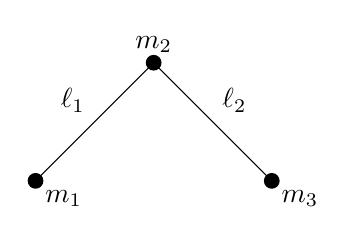
\begin{tikzpicture}
        \fill[black] (-1.5, -1.5) circle (1mm) node[anchor=north west] {$m_1$};
        \fill[black] (0, 0) circle (1mm) node[anchor=south] {$m_2$};
        \fill[black] (1.5, -1.5) circle (1mm) node[anchor=north west] {$m_3$};
        \draw (0, 0) -- node[anchor=south east] {$\ell_1$} (-1.5, -1.5);
        \draw (0, 0) -- node[anchor=south west] {$\ell_2$} (1.5, -1.5);
    \end{tikzpicture}
    \caption{Figure}
    \label{fig:over}
\end{figure}

$$q = \begin{bmatrix}
    r_1\\r_2\\r_3
\end{bmatrix}=\begin{bmatrix}
    x_1\\y_1\\x_2\\y_2\\x_3\\y_3
\end{bmatrix}$$
$$D(\mathcal{G})=\begin{bmatrix}
    I_{2\times2} & 0\\ -I_{2\times2} & I_{2\times2}\\ 0 & -I_{2\times2}
\end{bmatrix}$$
$$L(\mathcal{G})=D(\mathcal{G})D(\mathcal{G})^T=\begin{bmatrix}
    I_{2\times2} & -I_{2\times2} & 0\\
    -I_{2\times2} & 2I_{2\times2} & -I_{2\times2}\\
    0 & -I_{2\times2} & I_{2\times2}
\end{bmatrix}$$
$$q^TL(\mathcal{G})q=\ell_1^2+\ell_2^2$$
$$h(q)=q^TL(\mathcal{G})q-\ell_1^2-\ell_2^2=0$$
$$\frac{dh}{dt}=2q^TL(\mathcal{G})\dot{q}=0$$
This is the constraint we will use in the form:
$$\alpha^T\dot{q}=0,\:\alpha=L(\mathcal{G})q$$
And the Euler-Lagrange equation:
$$M\ddot{q}+Mg_6=f+\alpha\lambda$$
where $g_6=\begin{bmatrix}
    0&g&0&g&0&g
\end{bmatrix}^T$, $f$ is the externally applied force at the generalized coordinates, and $\alpha\lambda$ is the constraint force.

$$\ddot{q}=-g_6+M^{-1}(f+\alpha\lambda)=-g_6+M^{-1}f+M^{-1}L(\mathcal{G})q\lambda$$
$$\alpha^T\ddot{q}+\dot{\alpha}^T\dot{q}=0$$
$$q^TL(\mathcal{G})\ddot{q}+\dot{q}^TL(\mathcal{G})\dot{q}=0$$
$$q^TL(\mathcal{G})(-g_6+M^{-1}f+M^{-1}L(\mathcal{G})q\lambda)+\dot{q}^TL(\mathcal{G})\dot{q}=0$$
\begin{align*}
    M\ddot{q}&+Mg_6+\left(\frac{\dot{q}^TL(\mathcal{G})\dot{q}-q^TL(\mathcal{G})g_6}{q^TL(\mathcal{G})M^{-1}L(\mathcal{G})q}\right)L(\mathcal{G})q\\
    &=\left(I-\frac{L(\mathcal{G})qq^TL(\mathcal{G})M^{-1}}{q^TL(\mathcal{G})M^{-1}L(\mathcal{G})q}\right)f
\end{align*}

The denominator kind of has an interesting structure:
$$q^TL(\mathcal{G})M^{-1}L(\mathcal{G})q$$
$$=q^TD(\mathcal{G})D(\mathcal{G})^TM^{-1}D(\mathcal{G})D(\mathcal{G})^Tq$$

Now, let $q_e=D(\mathcal{G})^Tq$ be the edge states associated with $\mathcal{G}$. The expression becomes:
$$q_e^TD(\mathcal{G})^TM^{-1}D(\mathcal{G})q_e$$
which kind of looks like the quadratic form of the weighted edge Laplacian with the inverse of the masses as weights.

Separate idea: can we use notions of leader-follower formation control to control a robotic system in which one or more bodies are grounded?

$$f=B(q)T=\begin{bmatrix}
    R_{90}\frac{r_1-r_2}{\|r_1-r_2\|} & 0_{2\times1}\\
    0_{2\times1} & 0_{2\times1}\\
    0_{2\times1} & R_{90}\frac{r_3-r_2}{\|r_3-r_2\|}
\end{bmatrix}\begin{bmatrix}
    T_1\\T_3
\end{bmatrix}$$
$$R_{90}=\begin{bmatrix}
    0 & -1\\ 1 & 0
\end{bmatrix}$$

\subsection{Prismatic Joint}
\begin{figure}[htbp]
    \centering
    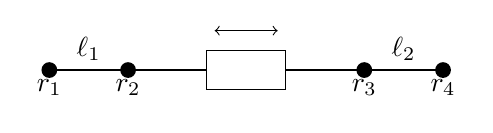
\begin{tikzpicture}
        \fill[black] (-2.5, 0) circle (1mm) node[anchor=north] {$r_1$};
        \fill[black] (-1.5, 0) circle (1mm) node[anchor=north] {$r_2$};
        \fill[black] (1.5, 0) circle (1mm) node[anchor=north] {$r_3$};
        \fill[black] (2.5, 0) circle (1mm) node[anchor=north] {$r_4$};

        \draw (-2.5, 0) -- node[anchor=south] {$\ell_1$} (-1.5, 0);
        \draw (2.5, 0) -- node[anchor=south] {$\ell_2$} (1.5, 0);
        \draw (-1.5, 0) -- (1.5, 0);
        \filldraw[fill=white, draw=black] (-0.5, 0.25) rectangle (0.5, -0.25);
        \draw[<->] (-0.4, 0.5) -- (0.4, 0.5);
    \end{tikzpicture}
    \caption{Figure}
    \label{fig:over2}
\end{figure}

$r_2-r_1$ is parallel to $r_4-r_3$ and pointing in the same direction, so:
$$(r_2-r_1)^T(r_4-r_3)=\|r_2-r_1\|\|r_4-r_3\|=\ell_1\ell_2$$
which can be rewritten as:
$$q^TL_1(\mathcal{G})q=2\ell_1\ell_2$$
where:
$$L_1(\mathcal{G})=\begin{bmatrix}
    0 & 0 & I_{2\times2} & -I_{2\times2}\\
    0 & 0 & -I_{2\times2} & I_{2\times2}\\
    I_{2\times2} & -I_{2\times2} & 0 & 0\\
    -I_{2\times2} & I_{2\times2} & 0 & 0
\end{bmatrix}$$

Also, length must be preserved:
$$(r_2-r_1)^T(r_2-r_1)=\ell_1^2$$
$$(r_4-r_3)^T(r_4-r_3)=\ell_2^2$$
$$q^TL_2(\mathcal{G})q=\ell_1^2+\ell_2^2$$
where:
$$L_2(\mathcal{G})=\begin{bmatrix}
    I_{2\times2} & -I_{2\times2} & 0 & 0\\
    -I_{2\times2} & I_{2\times2} & 0 & 0\\
    0 & 0 & I_{2\times2} & -I_{2\times2}\\
    0 & 0 & -I_{2\times2} & I_{2\times2}
\end{bmatrix}$$

Let $L(\mathcal{G})=L_1(\mathcal{G})+L_2(\mathcal{G})$
$$h(q)=q^TL(\mathcal{G})q-2\ell_1\ell_2-\ell_1^2-\ell_2^2=0$$
$$\frac{dh}{dt}=2q^TL(\mathcal{G})\dot{q}=0$$
So,
$$L(\mathcal{G})=\begin{bmatrix}
    I_{2\times2} & -I_{2\times2} & I_{2\times2} & -I_{2\times2}\\
    -I_{2\times2} & I_{2\times2} & -I_{2\times2} & I_{2\times2}\\
    I_{2\times2} & -I_{2\times2} & I_{2\times2} & -I_{2\times2}\\
    -I_{2\times2} & I_{2\times2} & -I_{2\times2} & I_{2\times2}
\end{bmatrix}$$

\begin{figure}[htbp]
    \centering
    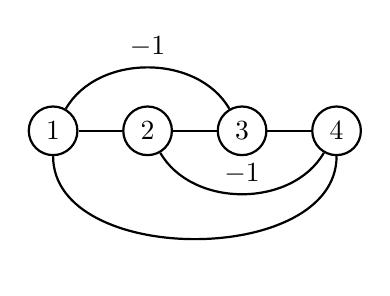
\begin{tikzpicture}[node distance={12mm}, thick, main/.style = {draw, circle}]
        \node[main] (1) {$1$};
        \node[main] (2) [right of=1] {$2$};
        \node[main] (3) [right of=2] {$3$};
        \node[main] (4) [right of=3] {$4$};
        \draw (1) -- (2);
        \draw (2) -- (3);
        \draw (3) -- (4);
        \draw (1) to [out=60, in=120] node[anchor=south] {$-1$} (3);
        \draw (2) to [out=-60, in=-120] node[anchor=south] {$-1$} (4);
        \draw (1) to [out=-90, in=-90] (4);
    \end{tikzpicture}
    \caption{Graph}
    \label{ting3}
\end{figure}

\subsection{Learning the network}
Given $n$ measurements of position and velocity, if we minimize the following function, we can find the best estimate of the graph Laplacian for a system.
$$\argmin_{L(\mathcal{G})}\sum_{i=1}^n(q_i^TL(\mathcal{G})\dot{q}_i)$$

\subsection{Trying again}
\begin{itemize}
    \item $n$ sets of coordinates (nodes)
    \item $k$ constraints (edges)
\end{itemize}

$$Q=\begin{bmatrix}
    x_1 & y_1\\
    \vdots & \vdots\\
    x_n & y_n
\end{bmatrix}\in\mathbb{R}^{n\times2},\:
G=\begin{bmatrix}
    0 & g\\
    \vdots & \vdots\\
    0 & g
\end{bmatrix}\in\mathbb{R}^{n\times2}$$
$$M=\begin{bmatrix}
    m_1\\
    & \ddots\\
    & & m_n
\end{bmatrix}\in\mathbb{R}^{n\times n}$$
$$F=\begin{bmatrix}
    f_{1,x} & f_{1,y}\\
    \vdots & \vdots\\
    f_{n,x} & f_{n,y}
\end{bmatrix}$$
$$M\ddot{Q}+MG+\Gamma=F$$

Constraints in terms of the graph
$$D(G)= \begin{bmatrix}
    | & & |\\
    d_1 & \hdots & d_k\\
    | & & |
\end{bmatrix}\in\mathbb{R}^{n\times k}$$
$$L_i(\mathcal{G})=d_id_i^T\in\mathbb{R}^{n\times n}$$
$$h_i(Q)=\Tr(Q^TL_i(\mathcal{G})Q)+c_i=0$$
$$\frac{dh_i}{dQ}=2Q^TL_i(\mathcal{G})$$
$$A(Q)\triangleq\frac{1}{2}\frac{dh}{dQ}=\begin{bmatrix}
    Q^TL_1(\mathcal{G})\\ \vdots\\ Q^TL_k(\mathcal{G})
\end{bmatrix}\in\mathbb{R}^{2k\times n}$$
$$\lambda=\begin{bmatrix}
    \lambda_1\\ \vdots\\ \lambda_k
\end{bmatrix}\in\mathbb{R}^{k\times 1}$$
\begin{align*}
    \Gamma&=A(Q)^T(\lambda\otimes I_{2\times2})\\
    &=\begin{bmatrix}
        Q^Td_1d_1^T\\ \vdots\\ Q^Td_kd_k^T
    \end{bmatrix}^T\begin{bmatrix}
        \lambda_1I_{2\times2}\\ \vdots\\ \lambda_kI_{2\times2}
    \end{bmatrix}\\
    &=\begin{bmatrix}
        d_1d_1^TQ & \hdots & d_kd_k^TQ
    \end{bmatrix}\begin{bmatrix}
        \lambda_1I_{2\times2}\\ \vdots\\ \lambda_kI_{2\times2}
    \end{bmatrix}\\
    &= \sum_{i=1}^k d_i\lambda_id_i^TQ\\
    &= D(\mathcal{G})\Lambda D(\mathcal{G})^TQ\\
    &= L_w(\mathcal{G})Q
\end{align*}

$$M\ddot{Q}+MG+D(\mathcal{G})\Lambda D(\mathcal{G})^TQ=F$$
$$\ddot{Q}=-G+M^{-1}(F-D(\mathcal{G})\Lambda D(\mathcal{G})^TQ)$$
The equivalent to the velocity constraint $A(q)\dot{q}=0$ in this case is:
$$\begin{bmatrix}
    \Tr(Q^TL(\mathcal{G})_1\dot{Q})\\
    \vdots\\
    \Tr(Q^TL(\mathcal{G})_k\dot{Q})
\end{bmatrix}=0$$
Take the derivative:
$$\begin{bmatrix}
    \Tr(Q^TL_1(\mathcal{G})\ddot{Q}+\dot{Q}^TL(\mathcal{G})_1\dot{Q})\\
    \vdots\\
    \Tr(Q^TL_k(\mathcal{G})\ddot{Q}+\dot{Q}^TL(\mathcal{G})_k\dot{Q})
\end{bmatrix}=0$$
$$\begin{bmatrix}
    \Tr(Q^TL_1(\mathcal{G})\ddot{Q})+\|\dot{Q}^Td_1\|^2\\
    \vdots\\
    \Tr(Q^TL_k(\mathcal{G})\ddot{Q})+\|\dot{Q}^Td_k\|^2
\end{bmatrix}=0$$

$$\begin{bmatrix}
    \Tr(Q^TL_1(\mathcal{G})M^{-1}(F-D(\mathcal{G})\Lambda D(\mathcal{G})^TQ))+\|\dot{Q}^Td_1\|^2\\
    \vdots\\
    \Tr(Q^TL_k(\mathcal{G})M^{-1}(F-D(\mathcal{G})\Lambda D(\mathcal{G})^TQ))+\|\dot{Q}^Td_k\|^2
\end{bmatrix}=0$$
$$\begin{bmatrix}
    \Tr(Q^TL_1(\mathcal{G})M^{-1}D(\mathcal{G})\Lambda D(\mathcal{G})^TQ)\\
    \vdots\\
    \Tr(Q^TL_k(\mathcal{G})M^{-1}D(\mathcal{G})\Lambda D(\mathcal{G})^TQ)
\end{bmatrix}$$
$$=\begin{bmatrix}
    \Tr(Q^TL_1(\mathcal{G})M^{-1}F)+\|\dot{Q}^Td_1\|^2\\
    \vdots\\
    \Tr(Q^TL_k(\mathcal{G})M^{-1}F)+\|\dot{Q}^Td_k\|^2
\end{bmatrix}$$
$$\begin{bmatrix}
    \Tr(D(\mathcal{G})^TQQ^TL_1(\mathcal{G})M^{-1}D(\mathcal{G})\Lambda)\\
    \vdots\\
    \Tr(D(\mathcal{G})^TQQ^TL_k(\mathcal{G})M^{-1}D(\mathcal{G})\Lambda)
\end{bmatrix}$$
$$=\begin{bmatrix}
    \Tr(Q^TL_1(\mathcal{G})M^{-1}F)+\|\dot{Q}^Td_1\|^2\\
    \vdots\\
    \Tr(Q^TL_k(\mathcal{G})M^{-1}F)+\|\dot{Q}^Td_k\|^2
\end{bmatrix}$$

Define the transformation $\Tdiag:\mathbb{R}^{k\times k}\to\mathbb{R}^k$ by
$$\Tdiag(A)=\Tdiag\left(\begin{bmatrix}
    a_{11} & \hdots & a_{1k}\\
    \vdots & \ddots & \vdots\\
    a_{k1} & \hdots & a_{kk}
\end{bmatrix}\right)=\begin{bmatrix}
    a_{11}\\ \vdots\\ a_{kk}
\end{bmatrix}$$

$$\begin{bmatrix}
    \Tdiag(D(\mathcal{G})^TQQ^TL_1(\mathcal{G})M^{-1}D(\mathcal{G}))^T\\
    \vdots\\
    \Tdiag(D(\mathcal{G})^TQQ^TL_k(\mathcal{G})M^{-1}D(\mathcal{G}))^T
\end{bmatrix}\lambda$$
$$=\begin{bmatrix}
    \Tr(Q^TL_1(\mathcal{G})M^{-1}F)+\|\dot{Q}^Td_1\|^2\\
    \vdots\\
    \Tr(Q^TL_k(\mathcal{G})M^{-1}F)+\|\dot{Q}^Td_k\|^2
\end{bmatrix}$$
If the constraints are independent, the matrix should be invertible:
$$\lambda=\begin{bmatrix}
    \Tdiag(D(\mathcal{G})^TQQ^TL_1(\mathcal{G})M^{-1}D(\mathcal{G}))^T\\
    \vdots\\
    \Tdiag(D(\mathcal{G})^TQQ^TL_k(\mathcal{G})M^{-1}D(\mathcal{G}))^T
\end{bmatrix}^{-1}$$
$$*\begin{bmatrix}
    d_1^TM^{-1}FQ^Td_1+\|\dot{Q}^Td_1\|^2\\
    \vdots\\
    d_k^TM^{-1}FQ^Td_k+\|\dot{Q}^Td_k\|^2
\end{bmatrix}$$
$$\lambda=\left(D(\mathcal{G})^TM^{-1}D(\mathcal{G})\odot Q_eQ_e^T\right)^{-1}\begin{bmatrix}
    f_{1e}^Tr_{1e}+\|\dot{r}_{1e}\|^2\\
    \vdots\\
    f_{ke}^Tr_{ke}+\|\dot{r}_{ke}\|^2
\end{bmatrix}$$
If we can cancel out the force terms within $\lambda$, we only need information of each bar's angular speed and the angle between adjacent bars to solve.

\subsection{Example}
\begin{figure}[htbp]
    \centering
    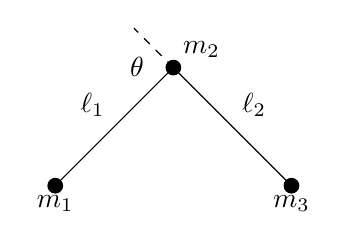
\begin{tikzpicture}
        \fill[black] (-1.5, -1.5) circle (1mm) node[anchor=north] {$m_1$};
        \fill[black] (0, 0) circle (1mm) node[anchor=south west] {$m_2$};
        \fill[black] (1.5, -1.5) circle (1mm) node[anchor=north] {$m_3$};
        \draw (0, 0) -- node[anchor=south east] {$\ell_1$} (-1.5, -1.5);
        \draw (0, 0) -- node[anchor=south west] {$\ell_2$} (1.5, -1.5);
        \draw[dashed] (0, 0) -- node[anchor=north east] {$\theta$} (-0.5, 0.5);
    \end{tikzpicture}
    \caption{Figure}
    \label{fig:overp}
\end{figure}
$$n=3,\:k=2$$
$$Q=\begin{bmatrix}
    x_1 & y_1\\
    x_2 & y_2\\
    x_3 & y_3
\end{bmatrix}=\begin{bmatrix}
    r_1^T\\ r_2^T\\ r_3^T
\end{bmatrix},\:
G=\begin{bmatrix}
    0 & g\\
    0 & g\\
    0 & g
\end{bmatrix}$$
$$M=\begin{bmatrix}
    m_1 & & \\
    & m_2 & \\
    & & m_3
\end{bmatrix},\:
F=\begin{bmatrix}
    f_1^T\\ f_2^T\\ f_3^T
\end{bmatrix}$$
$$M\ddot{Q}+MG+\Gamma=F$$
$$D(\mathcal{G})=\begin{bmatrix}
    1 & 0\\
    -1 & 1\\
    0 & -1
\end{bmatrix}$$
$$L_1(\mathcal{G})=\begin{bmatrix}
    1 & -1 & 0\\
    -1 & 1 & 0\\
    0 & 0 & 0
\end{bmatrix}$$
$$L_2(\mathcal{G})=\begin{bmatrix}
    0 & 0 & 0\\
    0 & 1 & -1\\
    0 & -1 & 1
\end{bmatrix}$$
\iffalse
$$A(Q)=\begin{bmatrix}
    Q^TL_1(\mathcal{G})\\ Q^TL_2(\mathcal{G})
\end{bmatrix}=\begin{bmatrix}
    x_1-x_2 & x_2-x_1 & 0\\
    y_1-y_2 & y_2-y_1 & 0\\
    0 & x_2-x_3 & x_3-x_2\\
    0 & y_2-y_3 & y_3-y_2
\end{bmatrix}$$
\begin{align*}
    \Gamma&=A(Q)^T(\lambda\otimes I_{2\times2})\\
    &=\begin{bmatrix}
        x_1-x_2 & y_1-y_2 & 0 & 0\\
        x_2-x_1 & y_2-y_1 & x_2-x_3 & y_2-y_3\\
        0 & 0 & x_3-x_2 & y_3-y_2
    \end{bmatrix}\begin{bmatrix}
        \lambda_1 & 0\\
        0 & \lambda_1\\
        \lambda_2 & 0\\
        0 & \lambda_2
    \end{bmatrix}\\
    &=\begin{bmatrix}
        \lambda_1(x_1-x_2) & \lambda_1(y_1-y_2)\\
        \lambda_1(x_2-x_1)+\lambda_2(x_2-x_3) & \lambda_1(y_2-y_1)+\lambda_2(y_2-y_3)\\
        \lambda_2(x_3-x_2) & \lambda_2(y_3-y_2)
    \end{bmatrix}
\end{align*}
\fi

Solve for $\lambda$ and substitute with edge variables:
$$Q_e=D(\mathcal{G})^TQ=\begin{bmatrix}
    (r_1-r_2)^T\\
    (r_2-r_3)^T
\end{bmatrix}=\begin{bmatrix}
    r_{1e}^T\\
    r_{2e}^T
\end{bmatrix}$$
\begin{align*}
    \lambda&=\begin{bmatrix}
        \left(\frac{1}{m_1}+\frac{1}{m_2}\right)\ell_1^2 & -\frac{1}{m_2}r_{1e}^Tr_{2e}\\
        -\frac{1}{m_2}r_{1e}^Tr_{2e} & \left(\frac{1}{m_2}+\frac{1}{m_3}\right)\ell_2^2
    \end{bmatrix}^{-1}\\
    &*\begin{bmatrix}
        r_{1e}^T\left(\frac{f_1}{m_1}-\frac{f_2}{m_2}\right)+\|\dot{r}_{1e}\|^2\\
        r_{2e}^T\left(\frac{f_2}{m_2}-\frac{f_3}{m_3}\right)+\|\dot{r}_{2e}\|^2
    \end{bmatrix}\\
    &=\frac{1}{\left(\frac{1}{m_1}+\frac{1}{m_2}\right)\ell_1^2\left(\frac{1}{m_2}+\frac{1}{m_3}\right)\ell_2^2-\left(\frac{1}{m_2}r_{1e}^Tr_{2e}\right)^2}\\
    &*\begin{bmatrix}
        \left(\frac{1}{m_2}+\frac{1}{m_3}\right)\ell_2^2 & \frac{1}{m_2}r_{1e}^Tr_{2e}\\
        \frac{1}{m_2}r_{1e}^Tr_{2e} & \left(\frac{1}{m_1}+\frac{1}{m_2}\right)\ell_1^2
    \end{bmatrix}\\
    &*\begin{bmatrix}
        r_{1e}^T\left(\frac{f_1}{m_1}-\frac{f_2}{m_2}\right)+\|\dot{r}_{1e}\|^2\\
        r_{2e}^T\left(\frac{f_2}{m_2}-\frac{f_3}{m_3}\right)+\|\dot{r}_{2e}\|^2
    \end{bmatrix}\\
    &=\frac{1}{\left(\frac{1}{m_1}+\frac{1}{m_2}\right)\ell_1^2\left(\frac{1}{m_2}+\frac{1}{m_3}\right)\ell_2^2-\left(\frac{1}{m_2}r_{1e}^Tr_{2e}\right)^2}\\
    &*\begin{bmatrix}
        \left(\frac{1}{m_2}+\frac{1}{m_3}\right)\ell_2^2\left(r_{1e}^T\left(\frac{f_1}{m_1}-\frac{f_2}{m_2}\right)+\|\dot{r}_{1e}\|^2\right) + \frac{1}{m_2}r_{1e}^Tr_{2e}\left(r_{2e}^T\left(\frac{f_2}{m_2}-\frac{f_3}{m_3}\right)+\|\dot{r}_{2e}\|^2\right)\\
        \frac{1}{m_2}r_{1e}^Tr_{2e}\left(r_{1e}^T\left(\frac{f_1}{m_1}-\frac{f_2}{m_2}\right)+\|\dot{r}_{1e}\|^2\right) + \left(\frac{1}{m_1}+\frac{1}{m_2}\right)\ell_1^2\left(r_{2e}^T\left(\frac{f_2}{m_2}-\frac{f_3}{m_3}\right)+\|\dot{r}_{2e}\|^2\right)
    \end{bmatrix}
\end{align*}

Simplifications:
$$\|r_{ie}\|=\ell_i$$
$$r_{1e}^Tr_{2e}=\ell_1\ell_2\cos\theta$$
For $\|\dot{r}_{1e}\|$, we consider the relative velocities of the masses. Let us write out: $\dot{r}_{1e}=\dot{r}_1-\dot{r}_2$. If we choose a reference frame to be at $m_2$, we can say $\dot{r}_{1e}'=\dot{r}_1'$. The $r_{1e}$ vector will always spin around the frame with constant radius, so there is a direct relationship between $\dot{r}_{1e}$ and the angular speed of the rotation of $\ell_1$ given by:
$$\|\dot{r}_{1e}\|^2=(\ell_1\omega_1)^2$$
where $\omega_1$ is the angular speed of the rotation of $\ell_1$ with respect to a frame fixed on $\ell_1$ (body frame).

\subsection{Add restrictions}
$$f_1\perp r_{1e},\:f_2=0,\:f_3\perp r_{2e}$$
\begin{multline} \label{eq:lambda}
    \lambda=\frac{1}{\left(\frac{1}{m_1m_2}+\frac{1}{m_1m_3}+\frac{1}{m_2m_3}+\frac{\sin^2\theta}{m_2^2}\right)\ell_1^2\ell_2^2}\\
    *\begin{bmatrix}
        \left(\frac{1}{m_2}+\frac{1}{m_3}\right)\ell_2^2\|\dot{r}_{1e}\|^2 + \frac{1}{m_2}r_{1e}^Tr_{2e}\|\dot{r}_{2e}\|^2\\
        \frac{1}{m_2}r_{1e}^Tr_{2e}\|\dot{r}_{1e}\|^2 + \left(\frac{1}{m_1}+\frac{1}{m_2}\right)\ell_1^2\|\dot{r}_{2e}\|^2
    \end{bmatrix}
\end{multline}
\begin{multline}
    \lambda=\frac{1}{\frac{1}{m_1m_2}+\frac{1}{m_1m_3}+\frac{1}{m_2m_3}+\frac{\sin^2\theta}{m_2^2}}\\*\begin{bmatrix}
        \left(\frac{1}{m_2}+\frac{1}{m_3}\right)\omega_1^2 + \frac{\ell_2}{m_2\ell_1}\cos\theta\omega_2^2\\
        \left(\frac{1}{m_1}+\frac{1}{m_2}\right)\omega_2^2 + \frac{\ell_1}{m_2\ell_2}\cos\theta\omega_1^2
    \end{bmatrix}
\end{multline}

\begin{align*}
    \Gamma&=D(\mathcal{G})\Lambda(\theta, \omega_1, \omega_2)D(\mathcal{G})^TQ\\
    &=\begin{bmatrix}
        \lambda_1r_{1e}^T\\
        -\lambda_1r_{1e}^T+\lambda_2r_{2e}^T\\
        -\lambda_2r_{2e}^T
    \end{bmatrix}
\end{align*}
We see that $\Gamma$ can be expressed entirely with edge variables. So, the only place where absolute variables are used in the full Euler-Lagrange equation is the $\ddot{Q}$ term, which means we can simplify the dynamics to $\ddot{Q}=\hdots$ with only knowledge of edge variables given a control $F$.

\subsection{Control}
\iffalse
Let's say the control goal is to cause $\theta\rightarrow0$. This is equivalent to $r_{1e}^Tr_{2e}\rightarrow\ell_1\ell_2$ (kind of but not really). This is where the network comes in handy because we only care about how the edge variables behave. We can write an error expression as:
$$-k_1(r_{1e}^Tr_{2e}-\ell_1\ell_2)-k_2(\dot{r}_{1e}^Tr_{2e}+r_{1e}^T\dot{r}_{2e})$$
\fi
Let's say the control goal is to cause $\theta\rightarrow180^\circ$ (bring the two rods together) and orient them in a specific direction, in this case make them flat. We specify the edge vectors to achieve: $r_{1e}\rightarrow\begin{bmatrix}
    \ell_1\\ 0
\end{bmatrix}$ and $r_{2e}\rightarrow\begin{bmatrix}
    -\ell_2\\ 0
\end{bmatrix}$ which is equivalent to:
$$Q_e\rightarrow Q_{e,d}$$
\begin{equation} \label{eq:Qe}
    Q_{e,d}=\begin{bmatrix}
        \ell_1 & 0\\
        -\ell_2 & 0
    \end{bmatrix}
\end{equation}
If this is the goal, we can write the feedback linearization as:
$$\ddot{Q}_e=-K_1\left(Q_e-Q_{e,d}\right)-K_2\dot{Q}_e$$
The Euler-Lagrange equation is:
$$M\ddot{Q}+MG+\Gamma=F$$
$$\ddot{Q}+G+M^{-1}\Gamma=M^{-1}F$$
$$D(\mathcal{G})^T\ddot{Q}+D(\mathcal{G})^TG+D(\mathcal{G})^TM^{-1}\Gamma=D(\mathcal{G})^TM^{-1}F$$
Now convert to edge states using the edge transformation $Q_e=D(\mathcal{G})^TQ$:
$$\ddot{Q}_e+D(\mathcal{G})^TM^{-1}\Gamma(Q_e, \dot{Q}_e)=D(\mathcal{G})^TM^{-1}F$$
\begin{multline} \label{eq:2}
    D(\mathcal{G})^TM^{-1}F=-K_1\left(Q_e-Q_{e,d}\right)-K_2\dot{Q}_e\\+D(\mathcal{G})^TM^{-1}\Gamma(Q_e, \dot{Q}_e)
\end{multline}
Now, if we have direct access to the weighted difference of force vectors on adjacent masses, we can control $Q_e$. We also have the freedom to add to the force vectors components that provide each mass with the same amount of acceleration without breaking this equation, meaning the robot can fight gravity while achieving relative consensus.

\subsection{Back to the example}
Let's say the force thrusters on $m_1$ and $m_3$ must be perpendicular to the rods and the thruster on $m_2$ is turned off. The scalars $u_1,\:u_2\in\mathbb{R}$ are the control inputs.
$$R_{90}=\begin{bmatrix}
    0 & -1\\ 1 & 0
\end{bmatrix}$$
$$f_1=u_1R_{90}\frac{r_{1e}}{\ell_1}$$
$$f_2=0$$
$$f_3=u_2R_{90}\frac{r_{2e}}{\ell_2}$$
The left side of equation \ref{eq:2} works out to:
$$D(\mathcal{G})^TM^{-1}F=\begin{bmatrix}
    u_1\frac{1}{m_1\ell_1}(R_{90}r_{1e})^T\\
    -u_2\frac{1}{m_3\ell_2}(R_{90}r_{2e})^T
\end{bmatrix}$$
We cannot choose this matrix arbitrarily given the constraints on the thruster directions, so we must project onto the workspace. Let the $i$th row of equation \ref{eq:2} take the form:
$$u_ia_i^T\approx b_i^T$$
The best solution for $u_i$ is:
$$u_i=\frac{a_i^Tb_i}{a_i^Ta_i}$$
Using this as the control force, we get the following solutions of $r_{1e}$ and $r_{2e}$ over time.

\begin{figure}[htbp]
    \centering
    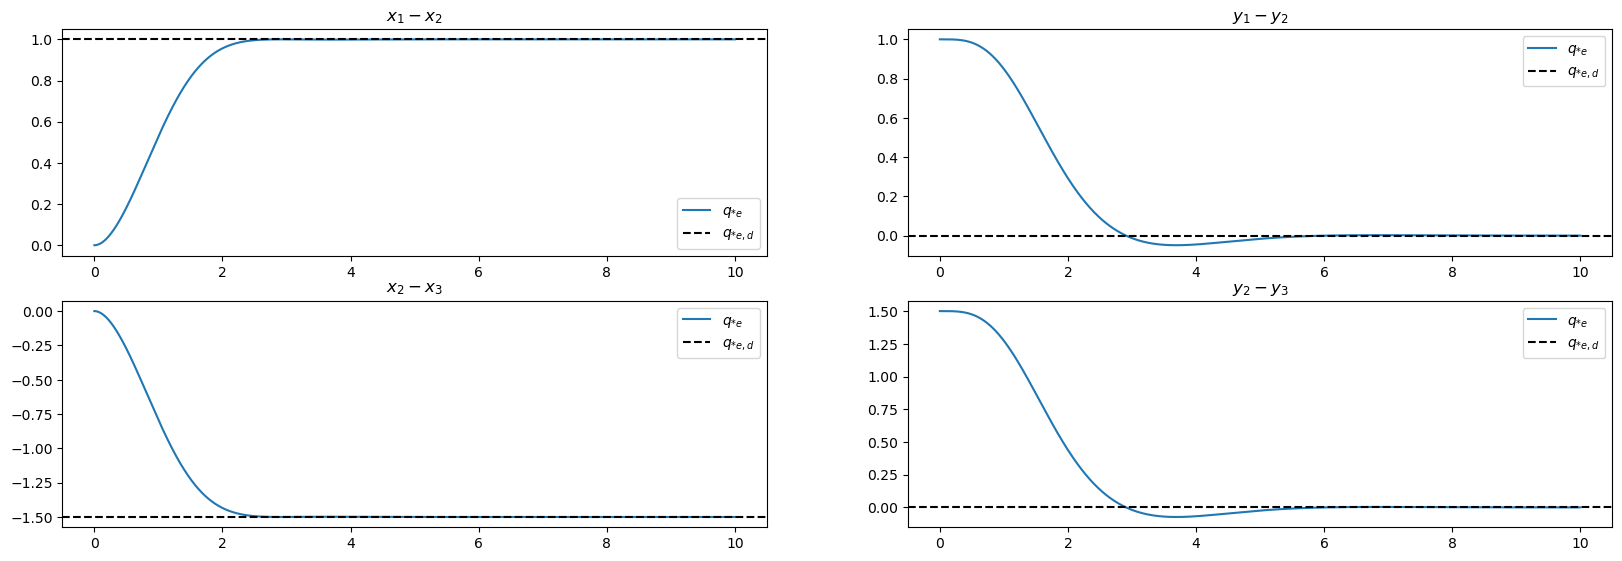
\includegraphics[width=0.48\textwidth]{fig2.png}
    \caption{Simulated edge states plot}
    \label{plots}
\end{figure}
In the simulation, $\ell_1=1$ and $\ell_2=1.5$, so the control objective from equation \ref{eq:Qe} is satisfied.
\begin{figure}[htbp]
    \centering
    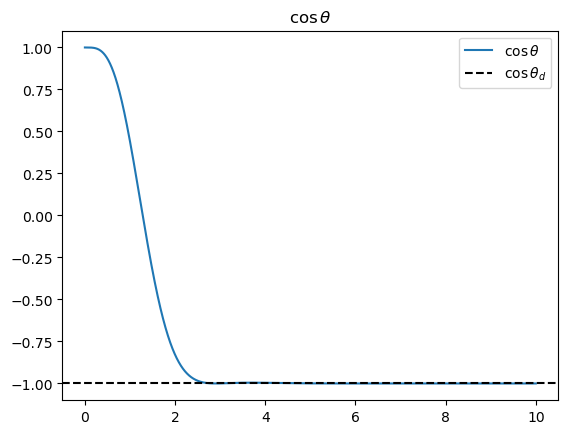
\includegraphics[width=0.48\textwidth]{cos.png}
    \caption{Simulated angle between rods}
    \label{plots1}
\end{figure}
\begin{figure}[htbp]
    \centering
    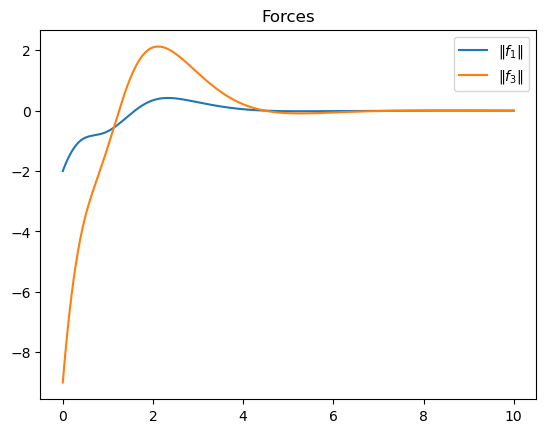
\includegraphics[width=0.48\textwidth]{forces.png}
    \caption{Simulated control forces}
    \label{plots2}
\end{figure}

\subsection{Closer look at the solution}
The control objective has been achieved when $Q_e=Q_{e,d}$ and $\dot{Q}_e=0$. Looking at equation \ref{eq:lambda}, we see that if $\dot{Q}_e=0$, then $\lambda=0$. The error terms in equation \ref{eq:2} will go to zero and the $\Gamma$ will also go to zero if $\lambda=0$. Therefore, it makes sense for the forces to converge to zero as the objective is achieved as seen in Figure \ref{plots2}. If $\dot{Q}_e$ is desired to be something other than zero (rods keep spinning at a desired frequency) then the forces would need to keep going.

Understand the solution better

The solution works for every combination of initial conditions and control objectives that I tried including 90 degree configurations and nonzero initial velocities that are feasible.

Lyapunov function

What if we remove all restrictions from $f_2$, but then place restrictions on $f_1$ and $f_3$ so that the force terms go away from $\lambda$?

Leader-follower network, 

Longer snake, is there a local network?

Mapping between difference of forces and a single force on the link.

\subsection{Longer snake}
$$D(\mathcal{G})=\begin{bmatrix}
    1 & 0 & 0\\
    -1 & 1 & 0\\
    0 & -1 & 1\\
    0 & 0 & -1
\end{bmatrix}$$

\subsection{Node control}
\begin{multline} \label{eq:f2}
    f_2=m_2(-k_3(r_2-r_{2,d}(t)) - k_4(\dot{r}_2-\dot{r}_{2,d}(t)) + \ddot{r}_{2,d}(t))\\
    + m_2\begin{bmatrix} 0\\ g \end{bmatrix}\\
    - \lambda_1(Q_{e,d},\dot{Q}_{e,d})r_{1e,d} + \lambda_2(Q_{e,d},\dot{Q}_{e,d})r_{2e,d}\\
\end{multline}
Note that equation \ref{eq:f2} only contains state information about $r_2$ and $\dot{r}_2$.

Gravity seems to be a really big issue to overcome.

\section{Summary}
\begin{itemize}
    \item Matrix differential form of the Euler-Lagrange equation
    \item Derivation of $\Gamma$ (constraint force vectors) and $\lambda$ (constraint force magnitudes)
    \item Example of simple overparameterized system with distance constraints 2-bar
    \item What info is needed for $\lambda$
    \item PD control of edge states
    \item Adding control of global variables with edge control (leader-follower)
    \item More examples: jointed wing, star, X-wing
\end{itemize}

\iffalse
\section*{References}

Please number citations consecutively within brackets \cite{b1}

\begin{thebibliography}{00}
\bibitem{b1} G. Eason, B. Noble, and I. N. Sneddon, ``On certain integrals of Lipschitz-Hankel type involving products of Bessel functions,'' Phil. Trans. Roy. Soc. London, vol. A247, pp. 529--551, April 1955.
\bibitem{b2} J. Clerk Maxwell, A Treatise on Electricity and Magnetism, 3rd ed., vol. 2. Oxford: Clarendon, 1892, pp.68--73.
\bibitem{b3} I. S. Jacobs and C. P. Bean, ``Fine particles, thin films and exchange anisotropy,'' in Magnetism, vol. III, G. T. Rado and H. Suhl, Eds. New York: Academic, 1963, pp. 271--350.
\bibitem{b4} K. Elissa, ``Title of paper if known,'' unpublished.
\bibitem{b5} R. Nicole, ``Title of paper with only first word capitalized,'' J. Name Stand. Abbrev., in press.
\bibitem{b6} Y. Yorozu, M. Hirano, K. Oka, and Y. Tagawa, ``Electron spectroscopy studies on magneto-optical media and plastic substrate interface,'' IEEE Transl. J. Magn. Japan, vol. 2, pp. 740--741, August 1987 [Digests 9th Annual Conf. Magnetics Japan, p. 301, 1982].
\bibitem{b7} M. Young, The Technical Writer's Handbook. Mill Valley, CA: University Science, 1989.
\end{thebibliography}
\vspace{12pt}
\fi

\end{document}
